\chapter{Discretization}
\label{chap:Discretization}

\section{Spatial discretization}
\label{sec:Spatial discretization}
GKV is a Vlasov (continuum) simulation code. The perpendicular directions are already given by a discrete representation in Fourier space $(k_x, k_y)$. The other three directions $(z,v_\parallel,\mu)$ are discretized by an equidistant grid. Defining box sizes $-L_x \leq \bar{x} < L_x, -L_y \leq \bar{y} < L_y, -L_z \leq \bar{z} < L_z, -L_v \leq \bar{v}_\parallel \leq L_v, 0 \leq \bar{\mu} \leq \frac{L_v^2}{2}$ and grid numbers $(2\mathtt{nx}+1,\mathtt{global\_ny}+1,2\mathtt{global\_nz},2\mathtt{global\_nv},\mathtt{global\_nm}+1)$ in $(k_x,k_y,z,v_\parallel,\mu)$, the grid of GKV is given by
\begin{align}
k_x &= \mathtt{mx} \Delta k_x ~~(-\mathtt{nx} \leq \mathtt{mx} \leq \mathtt{nx}), \nonumber \\
k_y &= \mathtt{my} \Delta k_y ~~(0 \leq \mathtt{my} \leq \mathtt{global\_ny}) \nonumber \\
z &= \mathtt{iz} \Delta z ~~(-\mathtt{global\_nz} \leq \mathtt{iz} \leq \mathtt{global\_nz-1}), \nonumber \\
v_\parallel &= -L_v + (\mathtt{iv}-1) \Delta v_\parallel ~~(1 \leq \mathtt{iv} \leq 2\mathtt{global\_nv}), \nonumber \\
\mu &= \frac{(\mathtt{im} \Delta w)^2}{2} ~~(0 \leq \mathtt{im} \leq \mathtt{global\_nm}), \nonumber
\end{align}
where $\Delta k_x = \frac{\pi}{L_x}, \Delta k_y = \frac{\pi}{L_y}, \Delta z = \frac{L_z}{\mathtt{global\_nz}}, \Delta v_\parallel = \frac{2L_v}{2\mathtt{global\_nv}-1}, \Delta w = \frac{L_v}{\mathtt{global\_nm}}$.

Derivatives in $(z,v_\parallel,\mu)$ are discretized by finite difference method, and then, GKV solves the $\delta f$ gyrokinetic equations, Eqs. (\ref{eq:vlasoveq_normalized})-(\ref{eq:ampereeq_normalized}), in $(k_x,k_y,z,v_\parallel,\mu)$ space, except for the nonlinear term. Since direct calculation of nonlinear convolution in wavenumber space is computationally expensive, the nonlinear term is evaluated in the real space, employing $(2\mathtt{nxw},2\mathtt{nyw},2\mathtt{global\_nz},2\mathtt{global\_nv},\mathtt{global\_nm}+1)$ grid points in $(x,y,z,v_\parallel,\mu)$, and is transformed back to the wavenumber space by means of 2D Fast Fourier Transform (FFT) algorithm and the 3/2 de-aliasing rule in $(k_x, k_y)$.

To implement the pseudo-periodic boundary condition along a field line, Eq. (\ref{eq:boundarycondition}), the shift of the radial wave number $\delta k_x (k_y) = - 2N_\theta \pi \hat{s} k_y$ as a function of $k_y$ should be equal to the integral multiple of the minimum radial wave number $\Delta k_x$. This gives a constraint between radial and field-line-label box sizes. In GKV, the minimum field-line-label wave number $\Delta k_y$ and the ratio $m = \left| \frac{\delta k_x (\Delta k_y)}{N_\theta \Delta k_x} \right|$ are given in the namelist (\texttt{kymin} and \texttt{m\_j}, respectively), and then, $\Delta k_x = |2\pi \hat{s} \Delta k_y / m|$, $L_x = \pi /\Delta k_x$, $L_y = \pi / \Delta k_y$.




\section{Temporal discretization}
\label{sec:Temporal discretization}

\subsection{i. Explicit implementation}
GKV usually uses 4th-order explicit Runge-Kutta-Gill method. \cite{Gill1951CPS}

\subsection{ii. Explicit collisionless physics and implicit collision implementation}

An alternative option is implicit collision solver which is useful for Lorentz or Sugama collision operators having velocity-dependent collision frequencies \cite{Maeyama2018CPC}. Splitting collisionless physics and collision operator by means of 2nd-order (Strang) operator split, the collisionless physics is solved by using 4th-order explicit Runge-Kutta-Gill method, while the collision operator is solved by using 2nd-order semi-implicit Crank-Nicolson method. Bi-CGSTAB method is used as an iterative matrix solver for implicit collision.





\section{Inter-node decomposition by using MPI}
\label{sec:Inter-node decomposition by using MPI}

The computations are parallelized by using the OpenMP/MPI hybrid parallelization which suites for hierarchical hardware of the nodes having a number of cores with a shared memory and connected by an interconnect network.

\begin{figure}[tb!]
  \centering
  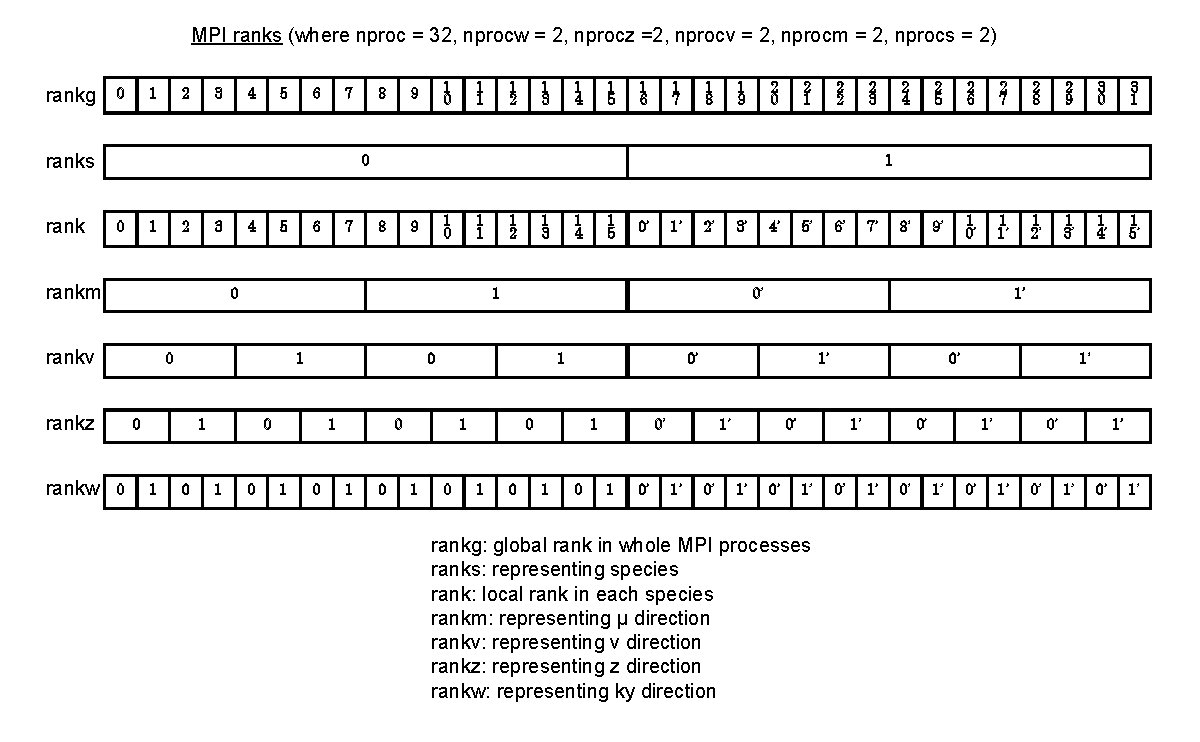
\includegraphics[scale=0.8]{./discretization/140627MPI_ranks_communicators_1.eps}
  \caption{An example of MPI ranks in GKV.}
  \label{fig:MPI_ranks_communicators_1}
\end{figure}
\begin{figure}[tb!]
  \centering
  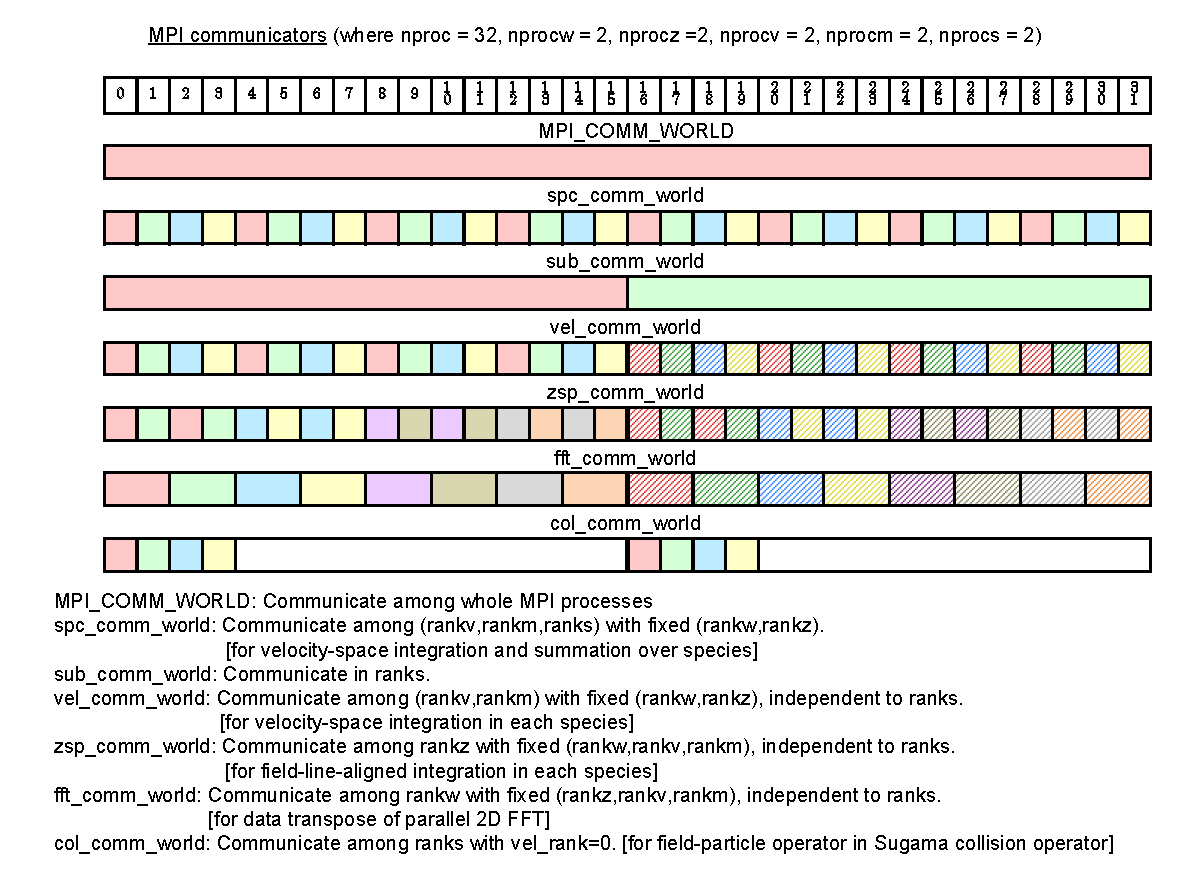
\includegraphics[scale=0.8]{./discretization/140627MPI_ranks_communicators_2.eps}
  \caption{An example of MPI communicators in GKV.}
  \label{fig:MPI_ranks_communicators_2}
\end{figure}
\begin{figure}[tb!]
  \centering
  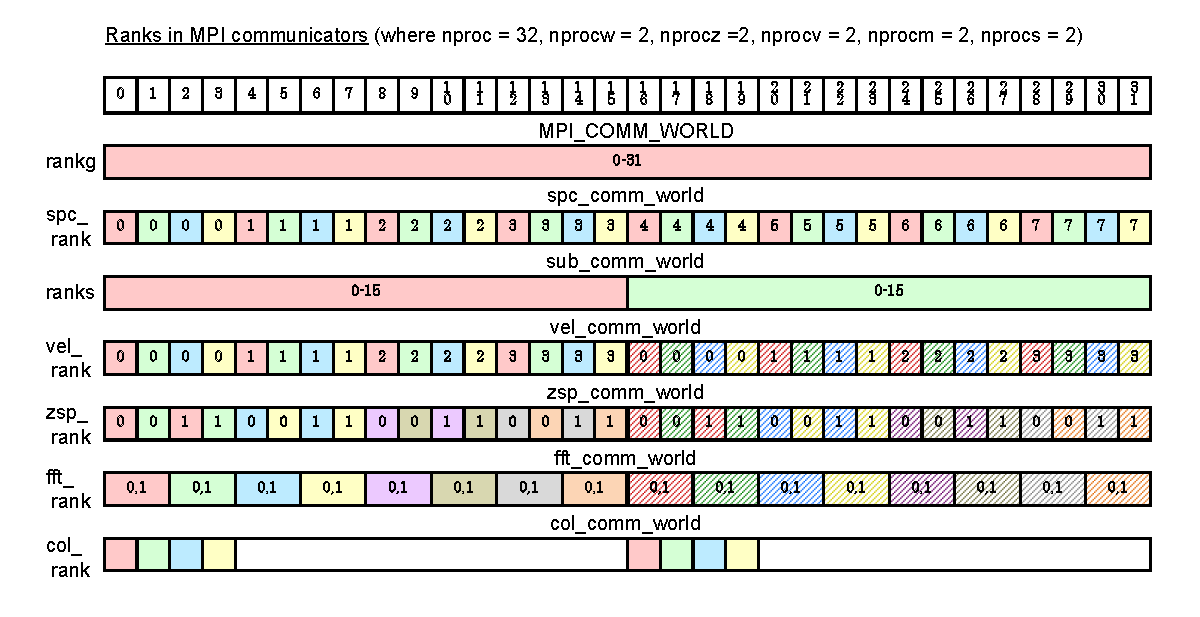
\includegraphics[scale=0.8]{./discretization/140627MPI_ranks_communicators_3.eps}
  \caption{An example of MPI ranks in communicators in GKV.}
  \label{fig:MPI_ranks_communicators_3}
\end{figure}
Taking advantage of the multi-dimensional problem, multi-dimensional domain decomposition is applied for $y$, $z$, $v_\parallel$, $\mu$ and $s$, where 2D FFTs in $x$ and $y$ are parallelized by means of the transpose split method. Then, the required MPI communications are data transpose for the parallel 2D FFTs in $x$ and $y$, point-to-point communications in $z$, $v_\parallel$ and $\mu$ for finite difference methods, and reduction communications over $v_\parallel$, $\mu$ and $s$ for velocity-space and species integration. Figures \ref{fig:MPI_ranks_communicators_1}-\ref{fig:MPI_ranks_communicators_3} show schematic pictures of the multi-layer structure of the multi-dimensional domain decomposition, illustrating the case that $y$, $z$, $v_\parallel$, $\mu$ and $s$ are respectively split by two MPI processes (and thus $2^5=32$ processes in total). Plasma species $s$ are decomposed as $\texttt{ranks} = 0, 1$, and each species are hierarchically decomposed by the magnetic moment $\mu$ (\texttt{rankm}), the parallel velocity $v_\parallel$ (\texttt{rankv}), the parallel direction $z$ (\texttt{rankz}), and the perpendicular direction $x,y$ (\texttt{rankw}). Thus, data transpose in $x$ and $y$ is performed for different subranks of \texttt{rankw} by using \texttt{fft\_comm\_world} communicator, point-to-point communications in $z$ ($v$ or  $m$)  are performed between \texttt{rankz} (\texttt{rankv} or \texttt{rankm}), while reduction communications over $v$, $\mu$ and $s$ are performed for fixed \texttt{rankz} and \texttt{rankw} by using \texttt{spc\_comm\_world} communicator.




\section{Intra-node decomposition by using OpenMP}
\label{sec:Intra-node decomposition by using OpenMP}
Intra-node decomposition is basically implemented by loop-level parallelization with OpenMP. Time-consuming MPI communications are masked by computation-communication overlap technique using MASTER thread. For more details, see Ref. \cite{Maeyama2015PC}.






\begin{thebibliography}{99}
\bibitem{Gill1951CPS}
  S. Gill,
  Proc. Cambridge Philosophical Soc. {\bf 47}, 96 (1951).
\bibitem{Maeyama2018CPC}
  S. Maeyama, T.-H. Watanabe, Y. Idomura, M. Nakata, and M. Nunami,
  Comput. Phys. Commun., submitted.
\bibitem{Maeyama2015PC}
  S. Maeyama, T.-H. Watanabe, Y. Idomura, M. Nakata, M. Nunami, and A. Ishizawa,
  Parallel Comput. {\bf 49}, 1 (2015).
\end{thebibliography}
